
%%%%%%%%%%%%%%%%%%%%%%% file typeinst.tex %%%%%%%%%%%%%%%%%%%%%%%%%
%
% This is the LaTeX source for the instructions to authors using
% the LaTeX document class 'llncs.cls' for contributions to
% the Lecture Notes in Computer Sciences series.
% http://www.springer.com/lncs       Springer Heidelberg 2006/05/04
%
% It may be used as a template for your own input - copy it
% to a new file with a new name and use it as the basis
% for your article.
%
% NB: the document class 'llncs' has its own and detailed documentation, see
% ftp://ftp.springer.de/data/pubftp/pub/tex/latex/llncs/latex2e/llncsdoc.pdf
%
%%%%%%%%%%%%%%%%%%%%%%%%%%%%%%%%%%%%%%%%%%%%%%%%%%%%%%%%%%%%%%%%%%%


\documentclass[runningheads,a4paper]{llncs}

\usepackage{amssymb}
\setcounter{tocdepth}{3}
\usepackage{graphicx}
\usepackage{float}
\usepackage[full]{complexity}
\usepackage{amsmath}
%\usepackage{amsfonts}
%\usepackage{amsthm}
\usepackage{subfigure}
%\usepackage{caption}
%\usepackage{subcaption}
%\usepackage{cite}
\usepackage{hyperref}
\usepackage{url}
%\usepackage{clrscode4e}
\usepackage{verbatim}
\urlstyle{same}
\newcommand{\keywords}[1]{\par\addvspace\baselineskip
\noindent\keywordname\enspace\ignorespaces#1}

% Uniform numbering for previously defined theorem environments (e.g., LNCS).
\makeatletter
\let\c@lemma=\c@theorem
\let\c@corollary=\c@theorem
\let\c@fact=\c@theorem
\makeatother

% Redefinition of LNCS or SODA or Springer proof environment to put a \Box at
% the end of every proof.
\let\realendproof=\endproof
\def\endproof{\hspace*{\fill}$\Box$\realendproof}

\begin{document}

\mainmatter  % start of an individual contribution

% first the title is needed
\title{The Fewest Clues Problem}

% a short form should be given in case it is too long for the running head
\titlerunning{The Fewest Clues Problem}

% the name(s) of the author(s) follow(s) next
%
% NB: Chinese authors should write their first names(s) in front of
% their surnames. This ensures that the names appear correctly in
% the running heads and the author index.
%
\author{Fermi Ma \and Ariel Schvartzman \and Erik Waingarten}
%
\authorrunning{Fermi Ma \and Ariel Schvartzman \and Erik Waingarten}
% (feature abused for this document to repeat the title also on left hand pages)

% the affiliations are given next; don't give your e-mail address
% unless you accept that it will be published
\institute{MIT,\\
77 Mass Ave., Cambridge, MA 02139, USA, \\
\protect\url{{fermima,arielsc,eaw}@mit.edu}}

%
% NB: a more complex sample for affiliations and the mapping to the
% corresponding authors can be found in the file "llncs.dem"
% (search for the string "\mainmatter" where a contribution starts).
% "llncs.dem" accompanies the document class "llncs.cls".
%

\maketitle

\section{Introduction}
\label{sec:introduction}

In 2012, McGuire, Tugermann, and Civario confirmed the conjecture that there are no uniquely solvable 16-clue Sudoku puzzles \cite{mcguire2012there}. It had long been known that 17 clues was sufficient, and there exists an online database containing over 50,000 such puzzles. Thus, the result by McGuire et al. completely solves the problem of determining the minimum number of Sudoku clues needed.

We consider a following generalization of the above Sudoku question: 
\begin{quote}
For any given problem, what is the fewest number of clues necessary to make it uniquely solvable?
\end{quote}

For example, if the problem is to find a Hamiltonian cycle in a given graph $G = (V,E)$, our question would be to determine the minimum number of edges you can specify before only one Hamiltonian cycle contains all of these edges. This general problem is motivated by possible applications to puzzle-making. 

A puzzle-maker for a newspaper might want to make a puzzle that contains as few clues as possible, but is still uniquely solvable (as the puzzle-maker might want to publish the answer in the next day's paper). The input to the problem is an idea of a partially filled puzzle, and the output is the least number of additional clues needed for the puzzle to be uniquely solvable.

We formalize this problem by defining the ``Fewest Clues Problem" ($\mathsf{FCP}$). We treat $\mathsf{FCP}$ as a new complexity class and show that its equivalence to $\Sigma_2$. We consider the idea of $\mathsf{FCP}$-hard problems, which in turn are also $\Sigma_2$ hard. We use this framework to analyze the $\mathsf{FCP}$ versions of classic $\NP$-hard problems such as SAT and 3SAT, as well as $\NP$-hard puzzle problems such as Latin square completion and Sudoku completion. 

The paper is organized as follows. In Section~\ref{sec:related}, we discuss previous research done on this sort of problem for the specific cases of Sudoku, Latin Squares, and graph coloring. We note that while this specific problem has been studied extensively, it is almost always done so with respect to a certain problem. In Section~\ref{sec:prelim}, we motivate and formally define the complexity class $\mathsf{FCP}$. We state what it means for a problem to be $\mathsf{FCP}$, and provide a framework for $\mathsf{FCP}$ reductions. In Section~\ref{sec:The Problems}, we consider $\mathsf{FCP}$ versions of the SAT, 3SAT, Triangle Partition, Latin Squares and Sudoku completion problems, and show why these problems are $\mathsf{FCP}$-hard. Then in Section~\ref{sec:relationship}, we show how the complexity class $\mathsf{FCP}$ fits into the landscape of well-known classes such as $\mathsf{P}, \mathsf{NP}, \Sigma_2^P$, and $\mathsf{PSPACE}$. Finally, in Section~\ref{sec:conclusion} we give concluding remarks and ideas for further research.

\section{Related Work}
\label{sec:relatedwork}

\section{The $\mathsf{FCP}$ Complexity Class}
\label{sec:complexityclass}

\subsection{Formalizing the Question}

In this section, we formalize the question of determining the fewest number of clues for a given instance of a problem. We will be working with $\NP$ search problems, this is the class of problems whose decision is in $\NP$, but we ask for a particular solution. In the case of Hamiltonian Path, instead of asking does there exists a Hamiltonian path, we are asking to present a Hamiltonian path. It is clear that $\NP$ search problems are ``harder" than decision problems, since one can answer the decision problem once one has found a solution.

In particular, we will have an $\NP$ search problem be comprised of a set of \emph{instances}, which will be strings over some finite alphabet. For a particular instance $x$, there is set of possible \emph{solutions}, which are strings of polynomial size with respect to $|x|$ over some finite alphabet. Each problem also comes with an algorithm $A$ that checks whether a string $s$ is in fact a solution for an instance $x$, which runs in polynomial time. This is the verifier. For a given language $L \in \NP$, $x \in L$ if and onll if $S(x)$ is non-empty.

A \emph{clue} will be an indexed character of a solution. So a clue indicates what character lies at some position of the solution.

\begin{definition}
Given some $\NP$ search problem $A$, the ``fewest clues" variation of $A$, $(\mathsf{FCP} A)$ asks for an instance of $A$, the minimum number of clues corresponding to a unique solution for any given instance.
\end{definition}

This set-up allows us to ask $\mathsf{FCP}$ variations to the common puzzles like Sudoku quiet easily. For the classical $9 \times 9$ Sudoku, we let the alphabet be $\Sigma = \{ 1, ..., 9 \} \cup \{ \Box \}$, and we let an instance be a string of length 81 with elements from $\Sigma$, where each position in the string corresponds to a position on the $9 \times 9$ Sudoku board. The presence of $\Box$ indicates that position is unknown. A solution will be a string of length $81$ with no $\Box$ characters. 

The algorithm $A$ checking whether a solution to some instance is correct. It does so by checking all three Sudoku rules: every row, column, and $3 \times 3$ inner-square contains all the numbers from $\{1 , ..., 9\}$. In addition, we check the solution contains the same numbers as the instance at the specified positions.

\begin{figure}
\centering
\label{fig:seventeencluesudoku}
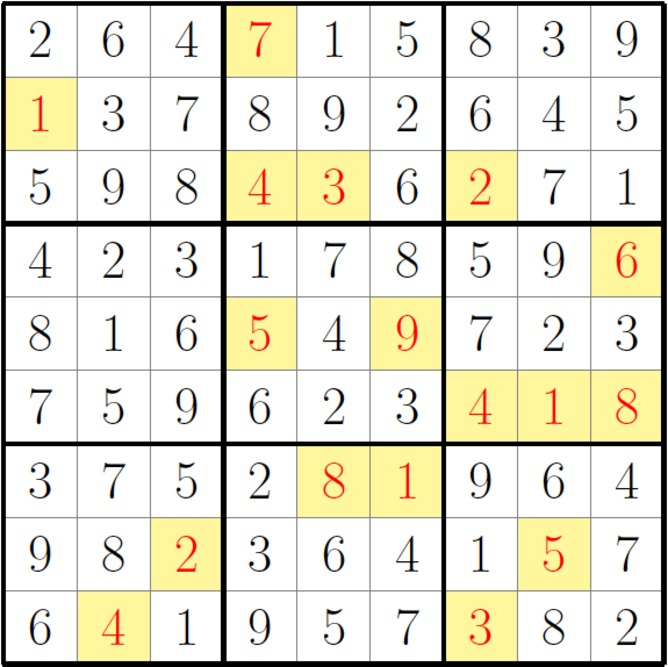
\includegraphics[width=0.5\linewidth]{seventeencluesudoku.jpg}
\caption{17-Clue $9 \times 9$ Sudoku, taken from \cite{smallsudoku}}
\end{figure}

The $\mathsf{FCP}$ Sudoku puzzle asks for a given starting point $x$ which is the fewest number of additional squares we must fill in order for the Sudoku to be uniquely solvable. A solution for the $9 \times 9$ case where the instance is initially empty is given in Figure~\ref{fig:seventeencluesudoku}. The fewest clues are given by the yellow squares.

We can also ask the corresponding decision question for some fewest clues problem: does there exist less than $k$ clues which uniquely specify a solution for a given instance? We can solve for the minimum number of clues necessary with a binary search through $k$ by asking the decision problem.

\subsection{The $\mathsf{FCP}$ Class}

We now present definitions that give rise to a complexity class, which we call  $\mathsf{FCP}$ (Fewest Clues Problem). This will sound very familiar to the above notions of solution and clue. We generalize the $\mathsf{FCP}$ variation to all $\NP$ search problems without having to explicitly specify the instance, solution and checker algorithm by framing the problem in terms of non-deterministic Turing machines. This generalization will give us an easy extension of the Cook-Levin theorem, which will show that $\mathsf{FCP}$ SAT is $\mathsf{FCP}$-complete. 

\subsubsection{Main Idea} We define the complexity class by defining a complete problem for the class. We will define a modified type of non-deterministic Turing machine which takes ``advice" for some non-deterministic steps. The advice will specify which branch of non-determinism to take. Then we will say that the complete problem is for a given non-deterministic Turing machine, whether the size of the smallest advice is less than $k$. This definition will allow us to easily show that any fewest clues problem corresponding to an $\NP$ search problem is contained in $\mathsf{FCP}$. 

We can assume without loss of generality that non-deterministic Turing machines (NTMs) have a branching factor of $2$ at each non-deterministic step. In addition, when the NTM performs a non-deterministic step where the computation branches, we assume that we have a canonical ordering of the two branches. We can call one the ``left" branch, and the other the ``right" branch. We also assume without loss of generality that all branches of the computation have length equal to a fixed polynomial since we are only dealing with $\NP$- search problems.

\begin{definition}
A partial certificate is a read-only tape which contains at each tape cell one of three possible characters, 0, 1, or $\bot$.
\end{definition}

\begin{definition}
The size of a partial certificate is the number of non-null entries. 
\end{definition}

For any $\NP$ search problem, a partial certificate is the generalization of a certificate. Also, any certificate of an $\NP$ problem can be thought of as a partial certificate. We think of partial certificates as ordinary certificates with some tape cells erased.

\begin{definition}
A modified non-deterministic Turing machine (mNTM) is an NTM where there is an additional input of a partial certificate. At each step of the computation, an mNTM reads the next tape cell of the partial certificate and if the partial certificate contains a 0, it takes the left branch of the computation. If it contains a 1, it takes the right branch of the computation. If it contains $\bot$, then it behaves non-deterministically. Other than that, an mNTM behaves exactly like an NTM.
\end{definition}

In some sense, a partial certificate makes an mNTM more deterministic. If a partial certificate contains no $\bot$ characters, then the mNTM behaves like a deterministic Turing machine. Alternatively, we can think of the partial certificate as feeding in clues to the mNTM in order to guide its computation. It is clear that given any NTM, we can construct a corresponding mNTM which runs in exactly the same manner, but has an additional input of a partial certificate. With these definitions, we are ready to define the class $\mathsf{FCP}$.

\begin{definition}
$\mathsf{FCP}$ is the class of function problems with the following complete problem:
\begin{quote}
Given an NTM running in polynomial time along with an input $x$, what is the size of the smallest a partial certificate such that the corresponding mNTM running on $x$ with the partial certificate has only one accepting branch?
\end{quote}
The corresponding decision version takes as additional input some $k$ and we ask whether the smallest partial certificate has size at most $k$.
\end{definition}

\begin{proposition}
Any problem in $\mathsf{FCP}$ can be phrased as a fewest clues problem.
\end{proposition}

\begin{proof}
Suppose we are given NTM $M$ which runs in polynomial time with respect to the length of the input. We create a fewest clues problem $\mathsf{FCP} M$:
\begin{itemize}
\item Instances: these are the instances of the NTM
\item Solutions: these are strings with characters in $\Sigma = \{ 0, 1 \}$ of length the runtime of $M$ on instance $x$ which indicate the branch leading to an accepting state.
\item Checker algorithm: Given an instance $x$ and a solution $s$, simulate an mNTM which corresponds to the NTM $M$ with partial certificate $s$. If the runtime of the mNTM is not equal to $|s|$, then reject. If it is equal, and so the mNTM behaves deterministically and accepts, then accept. 
\end{itemize}
Each clue of $\mathsf{FCP} M$ corresponds to a character in the partial certificate. Therefore, a set of clues corresponds to a partial certificate. If $C$ is a set of clues that has a unique solution, then the corresponding partial certificate will have a unique accepting branch. The smallest set of clues with a unique solution will therefore correspond to the smallest partial certificate with a unique accepting branch.

\begin{comment}
% more in detail.
\begin{enumerate}
\item Each clue in $\mathsf{FCP} M$ corresponds to a character in the certificate.\\
Proof: This is because each clue is an indexed character of the solution, which is in turn an indexed character of a certificate.
\item A set of clues corresponds to a partial certificate for $M$.\\
Proof: This follows from $1$ by taking many of characters in the certificate.
\item If $C$ is a set of clues with a unique solution, then the corresponding partial certificate will have a unique accepting branch.\\
Proof: Suppose there is another accepting branch in the mNTM. The non-deterministic turns at each step specify two possible solutions for the set of clues $C$. 
\item If $C$ is the smallest set of clues with a unique solution, then the corresponding partial certificate is the smallest partial certificate with mNTM having a unique accepting branch.\\
Proof: Follows from 3 and the fact that the size of the partial certificate is the same as the number of clues.
\item Therefore, a problem in $\mathsf{FCP}$ can be phrased as a fewest clues problem.\\
Proof: follows from $4$ and because each partial certificate corresponds to a set of clues.
\end{enumerate}
\end{comment}
\end{proof}

\begin{proposition}
\label{prop:fewesttofcp}
Any fewest clues problem with solution alphabet $\Sigma = \{ 0 ,1 \}$ is in $\mathsf{FCP}$.
\end{proposition}

\begin{proof}
We assume that we have some fewest clues problem, $\mathsf{FCP} A$, where:
\begin{itemize}
\item The set of instances is $I$.
\item The set of solutions is $S(x)$ for each $x \in I$ where each string is a character from some alphabet $\Sigma$ and each $s \in S(x)$ has $|s| \leq p(|x|)$.
\item We have an algorithm $A$ with inputs $x \in I$, $s \in S$ that decides in polynomial time whether $s$ is a solution to $x$.
\end{itemize}
We will construct a NTM $M$ such that the smallest partial certificate for $M$ will correspond to the fewest clues in $\mathsf{FCP} A$. \\
NTM $M$: Given an instance $x$, non-deterministically, for $p(|x|)$ steps, generate a solution $s$ by writing a character in each step, where the left branch writes $0$ in the solution and the right branch writes $1$ in the solution. Then simulate $A$ with inputs $x$ and $s$. Accept if $A$ accepts, and reject if $A$ rejects. 

The partial certificate only applies to non-deterministic steps, where $M$ writes down a solution. Therefore, a partial certificate tells the mNTM which characters to write at which positions deterministically, which correspond to a set of clues. So a partial certificate corresponds to a set of clues of the same size. Note that a partial certificate has an mNTM with only one accepting branch if and only if the corresponding set of clues has a unique solution. Therefore, the smallest partial certificate with a unique accepting branch will correspond to the smallest set of clues with a unique solution.
\begin{comment}
% more detail
\begin{enumerate}
\item A partial certificate corresponds to a set of clues of the same size.\\
Proof: The partial certificate only applies to non-deterministic steps, where $M$ writes down a solution. Therefore, a partial certificate tells the mNTM which characters to write at which positions deterministically, which correspond to a set of clues.
\item If a partial certificate has an mNTM with only one accepting branch, then the corresponding set of clues has a unique solution.\\
Proof: If the partial certificate has only one accepting branch, then it means that the corresponding set of clues have only a unique way to complete the clues to have a solution, since each branch explores every possible solution which is a superset of the set of clues.
\item If there exists a set of clues with a unique solution, there exists a partial certificate with only one accepting branch.\\
Proof: The set of clues specifies a partial certificate. If there is one way to fill the set of clues to have a solution, each solution will correspond to a branch of the computation. 
\item The smallest partial certificate with a unique accepting branch in the mNTM is the smallest set of clues with a unique solution.\\
Proof: follows from 2 and 3 and the fact that corresponding partial certificates and sets of clues have the same size. 
\end{enumerate}
\end{comment}
\end{proof}

We are almost there, we just need to show that the condition that $\Sigma = \{ 0, 1\}$ is unnecessary. The only problem with the above proof for arbitrary \emph{finite} $\Sigma$ is that we simply cannot write down every possible solution in $p(|x|)$ non-deterministic steps. Let $|\Sigma| = \sigma$. If we require the NTM $M$ to have branching factor $2$, it will take at least $\log \sigma$ non-deterministic steps to specify a unique character in $\Sigma$ to write down. This is a problem, since a specific character in the partial certificate might not be a clue, but rather might say, ``the $i$th character of the solution is in the first half of $\Sigma$". We would no longer maintain the number of clues equal to the size of the partial certificate, since each clue would correspond to $\log \sigma$ characters in a partial certificate. 

Instead of taking $\log \sigma$ steps to decide which character of $\Sigma$ to write in the solution, we use $\sigma$ steps. Then we show that a only one character in the partial certificate will be needed, and this character will correspond to a clue.

\begin{proposition}
Any fewest clues problem is in $\mathsf{FCP}$.
\end{proposition}

\begin{proof}
We will have the same construction as Proposition~\ref{prop:fewesttoffcp}, but instead of doing one non-deterministic step, we will use $\sigma$ non-deterministic steps to write a character in the solution.

The first non-deterministic step will choose whether or not to write the first element of $\Sigma$. The second will choose whether or not to write the second. The third step will choose the third element of $\Sigma$ and so on (see Figure~\ref{fig:branching}). Since each branch of the computation must be the same length, once we pick, we continue branching for $\sigma$ steps, and if we ever take a right branch again, will reject. The proof follows from these short claims:
\begin{enumerate}
\item Each clue corresponds to a segment of $\sigma$ characters in a certificate.\\
Proof: This is obvious, since it takes us $\sigma$ non-deterministic steps to make a choice of character.
\item There are exists a smallest partial certificate with a unique accepting branch with no 0's.\\
Proof: Suppose there was a 0 in the smallest partial certificate with a unique accepting branch, then that 0 corresponds to a taking some left branch. The left branch was in the process of picking some character, and suppose the unique accepting branch picked $a \in \Sigma$, then replace the 0 in the partial certificate, with the $1$ which picked $a$ in that segment of $\sigma$ branches. This is also a partial certificate of the same size. 
\item There is at most one character with a 1 in the smallest partial certificate for each chunk of $\sigma$ non-deterministic steps. So assume that all smallest partial certificates contain no zeros and a single one in each chunk of $\sigma$ characters.\\
Proof: if there were two 1's inside the chunk, the branch will reject.
\item If the $i$th non-deterministic step of the $j$th chunk took the right branch in the smallest partial certificate, then the fewest clue of picking the $i$th element of $\Sigma$ for index $j$ in the solution.\\
Proof: follows from the fact that there are only 1's, each in their $\sigma$ long chunks.
\item Each smallest partial certificate with unique accepting branch corresponds to a set of clues of the same size with a unique solution. \\
Proof: this follows from 4 and the fact that we know how to go from clues to partial certificates.
\end{enumerate}
\end{proof}

\begin{figure}
\centering
\label{fig:branching}
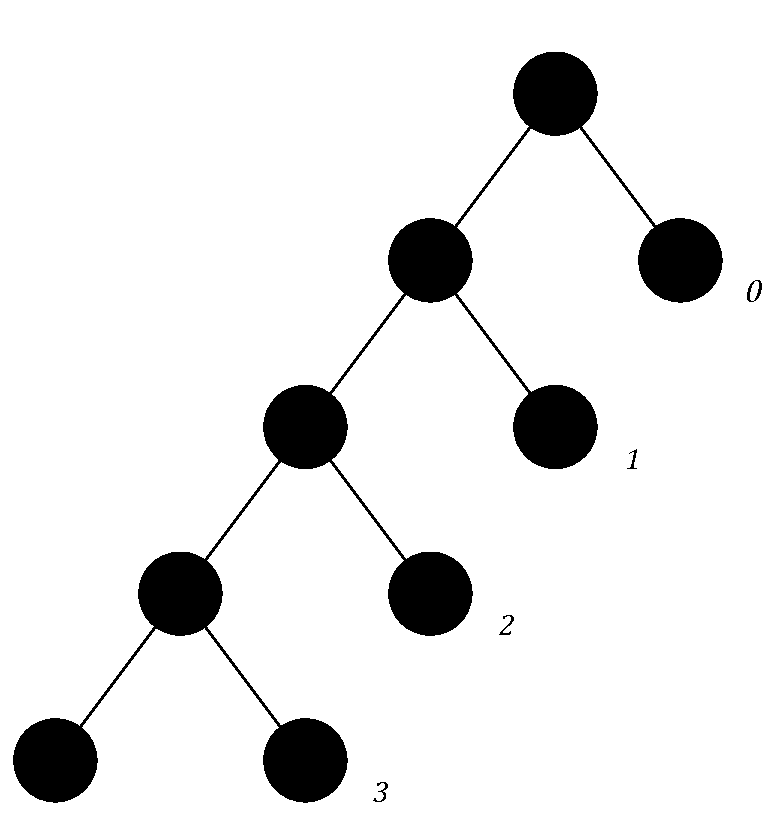
\includegraphics[width=0.4\linewidth]{branching.pdf}
\caption{Branching to pick $\Sigma = \{ 0, 1, 2, 3 \}$}
\end{figure}

The above proposition justifies our analysis of this class for answering these questions.

\subsection{$FCP-SAT$}

\section{$FCP = \Sigma_2$}

Having established given some complete problems for $\mathsf{FCP}$, we can ask where the complexity class lies in the context our current knowledge of complexity classes. We will be looking at the decision version of $\mathsf{FCP}$. 

\begin{proposition}
\label{prop:fcpsigma2}
$\mathsf{FCP} \subset \Sigma_2$
\end{proposition}

\begin{proof}
We give a formulation of the fewest clues problem in terms of a $\Sigma_2$ question. For a given problem $A$,
\[ (x, k) \in \mathsf{FCP} A \leftrightarrow \exists c, S \forall S' \phi(x, k, c, S, S') \]
Where $\phi$ checks that $c$ is a clue of size at most $k$, $c \subset S$, $S' \neq S$, $S$ is a solution to $x$ and $S'$ is not. This corresponds to asking for a set of clues $c$ of size at most $k$, which has a solution, $S$, but no other solution.  
\end{proof}

We now wish to show that $\Sigma_2 \subset \mathsf{FCP}$. We take the following $\Sigma_2$ complete problem: $\exists x \forall y \phi(x,y) = 0$. We will write this problem as an equivalent $\mathsf{FCP} SAT$ question: for a given $\phi$, does there exists a setting of $k$ variables, such that for any setting of the rest, there is one unique solution.

First, we take care of the unique solution. Suppose we had a modified question, $USAT$:
\begin{quote} 
Given some $\phi$, does there exists a setting of variables $x$ such that for any setting of varaibles $y$, there is one unique solution? 
\end{quote}

\begin{lemma}
$USAT$ is $\Sigma_2$ hard.
\end{lemma}

\begin{proof}
We will show that 
\[ \exists x \forall y \phi(x,y) = 0 \leftrightarrow \exists x \forall y, z \left(\phi'(x, 0, 0) = 1 \right) \wedge \left((y \neq 0 \vee z \neq 0 ) \rightarrow \phi'(x, y, z) = 0 \right) \]
The left-hand side is the complete problem of alternating $SAT$ for $\Sigma_2$, and the right-hand side says that $\phi'$ has only one solution for a given setting of $x$, $y=0$ and $z =0$. 

Asking $USAT$ for $\phi'$ would solve the alternating $SAT$ question. 

We let 
\begin{align}
\phi'(x, y, z) &= C_1 \vee C_2 \\
		    C_1 &=\left(\phi(x, y) \wedge (z = 1)\right) \\
		   C_2 &=  \left( y = 0 \wedge z = 0 \right) 
\end{align}
Note that $\phi'(x, 0, 0) = 1$. If $\exists x \forall y \phi(x, y)= 0$, then there is a setting of $x$ such that the $C_1 = 0$. The only way to satisfy $\phi'$ is through setting $y = 0$ and $z = 0$. If for any setting of $x$, there exists a setting of $y$ such that $\phi(x, y) = 1$, then we have some setting of $\phi'(x, y, 1) = 1$. So USAT would also be false since that assignment as well as $x, 0, 0$ evaluate to true.
\end{proof}

\begin{proposition}
\label{prop:fcpsatsigmacomp}
$\mathsf{FCP} SAT$ is $\Sigma_2$ hard.
\end{proposition}

\begin{proof}
We will reduce from $USAT$. For a given $\phi(x, y)$ with $|x| = k$, we ask, does there exists a setting of $2k$ variables such that $\phi'(x, x', y) = \phi(x, y) \vee \bigvee_i (x_i = x_i')$ has a unique solution?

Suppose $\exists x \forall y \phi(x,y)$ has a unique solution with assignment $\hat{x}$. Then we let $x = \hat{x}$, and for all $i$, we let $x_i' \neq x_i$. Therefore, once we set this, $\phi'(x, x', y)$ has a unique solution. 

Suppose for any setting of $x$, there is more than one setting of $y$'s to get a satisfying assignment, so $\phi(x, y) \notin USAT$. Then if from the $2k$ elements, we set $x$ and $x'$, we are fine, since there will be more than one setting of the $y$'s to satisfy $\phi'$. However, if we set some element not in $x$ or $x'$, then since we can only set $2k$, there will be some $x_i$ or $x_i'$ that is not set. So setting $x_i = x_i'$ will allow an arbitrary setting of the remaining variables, so also, $\phi'$ does not have a unique satisfying assignment.
\end{proof}

\begin{theorem}
$\mathsf{FCP} = \Sigma_2$
\end{theorem}

\begin{proof}
By Proposition~\ref{prop:fcpsigma2}, we know that $\mathsf{FCP} \subset \Sigma_2$. In addition, we showed in Proposition~\ref{prop:fcpsatsigmacomp} that $\mathsf{FCP} SAT$ is $\Sigma_2$ hard. Since $\mathsf{FCP} SAT$ is $\mathsf{FCP}$-complete, $\Sigma_2$ complete problems are also $\mathsf{FCP}$-complete, and so $\Sigma_2 \subset \mathsf{FCP}$. Therefore, $\mathsf{FCP} = \Sigma_2$. 
\end{proof}

\section{$\mathsf{FCP}$-Complete Problems}

\subsection{Reductions}

We define a special type of reductions that will allow us to show problems are $\mathsf{FCP}$-complete. 

\subsubsection{General Clue Reduction}
We need a function mapping instances of $A$ to instances of $B$, $f: I_A \rightarrow I_B$ such that $x \in A \iff f(x) \in B$. This is the usual definition of a reduction. We also want a function $g$ mapping the clues of $B$ to clues of $A$. We require that $g$ is surjective, $g$ is a bijection on solutions, and subsets are preserved. So $c \subset c' \iff g(c) \subset g(c')$. We also require that if $c$ is a clue set for $f(x)$, then $g(c)$ is a clue set for $x$. All these functions are computable in polynomial time.

So on input $x$, we find the minimum clue problem for $f(x)$, $c_{f(x)}$ and then use $g$ to get a clue $c_x$ for $x$.  

\begin{theorem}
Suppose $A$ reduces to $B$ with a general clue reduction and $\mathsf{FCP} A$ is $\mathsf{FCP}$-hard, then $\mathsf{FCP} B$ is $\mathsf{FCP}$-hard. 
\end{theorem}

\begin{proof}
We want to show that if $c_{f(x)}$ is a minimum clue set, then $g(c_{f(x)})$ is a minimum clue set as well.

First, we show that $g(c_{f(x)})$ is a clue. This is true because $c_{f(x)}$ is a clue. That is, there exists some solution $S_{f(x)}$ such that $c_{f(x)} \subset S_{f(x)}$, which means that $g(c_{f(x)}) \subset g(S_{f(x)})$, which is a solution.

Second, we need to show that $g(c_{f(x)})$ has a unique superset solution. Suppose there were two different solutions, $S_x^{(1)}$ and $S_{x}^{(2)}$, then $g(c_{f(x)}) \subset S_x^{(1)}, S_x^{(2)}$. This implies $c_{f(x)} \subset S_{f(x)}^{(1)}, S_{f(x)}^{(2)}$ because $g$ is surjective, and because solutions have inverses. Therfore, $c_{f(x)}$ is not unique.

Third, we need to show that $g(c_{f(x)})$ is minimal. Suppose there was some other $c' \subset g(c_{f(x)})$, since the $g$ is surjective, there exists some other $c_{f(x)}' \subset c_{f(x)}$ which is smaller. So by assumption, this must have two distinct solutions. But then mapping them again gives us two distinct solutions for $c'$. 

Therefore, $g(c_{f(x)})$ is a minimal clue set with a unique superset solution for $x$.
\end{proof}

\subsection{3SAT}

\begin{theorem}
$\mathsf{FCP}-3SAT$ is $\mathsf{FCP}$-complete. 
\end{theorem} 

\begin{proof}
We reduce from $\mathsf{FCP} 3SAT$ via a general clue reduction. We will define a recursive mapping $f$ from instances of SAT to those of 3-SAT. Suppose we are given a SAT formula $\phi$ with clauses $C_i$. If $|C_i| \leq 3$, then we preserve the clause. Otherwise, if $C_i$ has $k$ variables $x_1,...,x_k$ we replace the original clause with 
\[ 
(x_1 \vee x_2 \vee z_2) \wedge (\overline{z_2} \vee \overline{x_2}) \wedge (z_2 \vee x_2) \wedge f(\overline{z_2}, x_3, ..., x_k) 
\]

where the last term indicates we keep recursing until each clause has at most $3$ variables. Note that on each step we reduce the number of variables in the longest clause by at least $1$, so after $O(n)$ steps (per clause) we will have a valid 3-SAT instance at the cost of adding variables and small clauses. It is not hard to see that the original clause and it's mapped version agree on solutions. Notice that by construction $x_i \iff \overline{z_i}$. 

Now I will define $g$. $g$ will take a clue for 3SAT, or a partial assignment of the variables in $f(\phi)$ and give a partial assignment of the variables in $\phi$, it does this by mapping each variable individually. $g$ is the identity on the $x_i$ variables, and $g$ maps $z_i$ to $\overline{x_i}$. We check the properties of $g$:
\begin{enumerate}
\item $g$ is surjective. If there is any clue of $\phi$, it is also a clue of $f(\phi)$. 
\item $g$ is bijective on solutions. An assignment of $f(\phi)$ gives the assignment for $\phi$, and that same assignment uniquely describes the assignments for $z_i$, so $g$ bijectively maps them.
\item $g$ preserves subsets. This comes from the fact that $g$ maps individual assignments of the variables. 
\end{enumerate}
\end{proof}

\begin{corollary}
Not-All-Equal 3SAT (NAE 3SAT) is $\mathsf{FCP}$-complete.
\end{corollary}

\begin{proof}
The reduction for 3SAT above also works for NAE 3SAT. $x_i = \overline{z_i}$ which means that no satisfying assignment will have all three literals true in a clause. 
\end{proof}

\subsection{TrianglePartition}

\subsection{Latin Squares}

\subsection{Sudoku}

\section{$\mathsf{FCP}$ Versions of Easy Problems}

We would like to be able to understand what happens to problems in general when their $\mathsf{FCP}$ versions are asked. 

\subsection{$\mathsf{FCP}$ 2SAT} 

\textbf{Problem:} Given an instance 2-CNF formula $\phi(x_1,x_2,\dots,x_n)$, does there exist a setting of $k$ variables so that the remaining formula is uniquely satisfiable.

\begin{proposition}
$\mathsf{FCP} 2SAT$ is in \NP.
\end{proposition}

\begin{proof}
The clue of size $k$ is the certificate. Since $2SAT$ can be satified in polynomial time, we can check whether there is a unique solution in polynomial time.
\end{proof}

\begin{theorem} 
$\mathsf{FCP} 2SAT$ is \NP-hard.
\end{theorem}

We reduce from the NP-hard problem of finding a minimum independent dominating set. The problem gives a graph $G = (V,E)$ and asks for the smallest subset of vertices $S \subseteq V$ such that $S$ is a minimum independent dominating set. To state the constraints more clearly, such a set $S$ has the property that every vertex has a vertex in $S$ adjacent to it (every vertex is dominated), and does not have any edges $(u,v)$ where $u,v \in S$ (independence). \\

\noindent\textbf{Problem:} Given a graph $G = (V, E)$. Does there exists $S \subset V$, with $|S| \leq k$ such that 
\begin{itemize}
\item $\forall v \in V$, either $v \in S$ or $(u, v) \in E$, $u \in S$ 
\item $u, v \in S$ implies that there is no edge between $u$ and $v$. 
\end{itemize}

The reduction works as follows. For each edge $(u,v)$, we add the constraint $(\neg u \vee \neg v)$ to the 2SAT formula. We claim that a minimum clue set for the resulting 2SAT formula consists of a setting of $k$ variables to be true, and that the variables in the clue correspond to a minimum independent dominating set. For the other direction, we claim that a minimum independent dominating set gives us a minimum clue set for the 2SAT formula, by simply setting all the variables corresponding to vertices in the set to be true.

We will need the following lemma.

\begin{lemma} Given a set of clues of size $k$ with $k_f > 0$ variables set to false, there exists another set of clues of size at most $k$ with strictly fewer than $k_f$ variables set to false.
\end{lemma}

\begin{proof} 
Consider a variable $x_i$ set to be false. Consider its set of neighbors $N(x_i)$, guaranteed to be non-empty via construction. First, consider the case where $N(x_i)$ contains nodes set to true. For each of the nodes $v \in N(x_i)$ that are set to true, a clue must either say that $v$ is true, or there must be a clue that implies that $v$ is true. No matter what, we can either remove $x_i$ or replace $x_i$ with a clue that one of its neighbors are true (CHECK THIS). It remains to consider the case where all the neighbors of $x_i$ are set to false. In this case, we can switch the clue that $x_i$ is set to false with a clue that $x_i$ is set to true, which will imply that all of its neighbors are false.
\end{proof}

Now, we show that a minimum clue assignment gives an independent dominating set of the same size. Suppose we have a minimum clue assignment for 2SAT. We first apply the lemma above repeatedly until there are no false clues. So if we have a variable that is part of the clue, it is set to be true and implies all of its neighbors are false. Thus, we will not have a clue for any of the neighbors, since setting a variable to be false does not imply anything. This gives the independence property. We have a dominating set as well, since if there exists a vertex where no neighbor is a clue, then we cannot possibly know that any neighbors are set to true (since clues can only imply that other vertices are false), and since true variables are the only ones that give implications, we cannot know what this vertex is. This would contradict the fact that we have a uniquely determined solution.

Now we show that an independent dominating set gives a clue assignment of the same size. Suppose we have a minimum independent dominating set. If we set each variable in the minimum independent dominating set to be true, then we know due to the fact that it is a dominating set that every variable will be implied. So we know that this is a valid clue set.

To complete the proof, we claim that a minimum clue assignment actually corresponds to a $\emph{minimum}$ independent dominating set. If this were not the case, and a smaller independent dominating set existed, then we could go backwards to get a strictly smaller clue assignment. This would be a contradiction. 

\subsection{Other P problems with NP-hard FCP versions}

(open)

\subsection{P problems with $\Sigma_2$-hard FCP versions}

(open)

\section{Conclusion}
\label{sec:conclusion}


\bibliography{references}
\bibliographystyle{splncs}
\end{document}
